Ohm's Law describes the amount of energy it takes to push some amount of charge through a resistor.  A reasonable analogy is a ball moving quickly as it approaches a patch of mud.  It starts off with some amount of kinetic energy, then as it moves through the mud, it starts to slow down, losing some portion of the kinetic energy it has, until it clears the puddle.

Unfortunately, our analogy breaks down a bit, since our electrons are moving at the same speed the entire time.  We are not siphoning off the kinetic energy of the electrons, but rather the energy stored in the electrical potential, or voltage.

Ohm's Law states that the voltage drop {\it over} a resistor is proportional to both the resistance, $R$, and the current {\it through} the resistor:
\begin{equation}
  \Delta V = iR
\end{equation}

There is emphasis placed on the words {\it over} and {\it through} due to how we measure the voltage and current in a resistor for Ohm's Law.  We do not care about the voltage at any one place, but rather only the change between the two ends.  Likewise, whatever current is present at any point on the resistor will be present for all of it.  Neither occurs at a single point, but rather describes the entire resistor.

% Figure of Resistor for Ohm's Law
\begin{figure}
   \centering
%  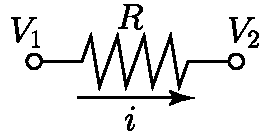
\includegraphics[width=0.5\linewidth]{figures/ohmsLaw}
  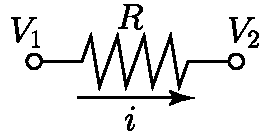
\includegraphics{figures/ohmsLaw}
  \caption{$\Delta V = V_1 - V_2$ for the circuit above, since energy is lost as charge passes through the resistor.}
  \label{fig:ohmsLaw}
\end{figure}

Looking at Figure \ref{fig:ohmsLaw}, you can see that we have labeled the two voltages on either side.  When we apply these voltages to $\Delta V$, we should always start on the tail end of our current (that is, the direction our current is coming from) and end on the head.  

Looking back to the pipe analogy from section \ref{sec:PrelimUnits}, $\Delta V$ is the loss of energy, $i$ is the flow rate through the thin pipe, and $R$ is how hard it is to get through the pipe.  More flow, whether fluid or electric, is more loss of energy, and a smaller pipe or larger resistance also means more loss.
